\documentclass[11pt,a4paper]{article}
\usepackage[utf8]{inputenc}
\usepackage[T1]{fontenc}
\usepackage[a4paper,margin=1in]{geometry}
\usepackage{lmodern}
\usepackage{amsmath,amssymb,mathtools}
\usepackage{graphicx}
\usepackage{caption}
\usepackage{subcaption}
\usepackage{enumitem}
\usepackage{hyperref}
\usepackage{booktabs}
\usepackage{microtype}
\usepackage{xcolor}
\usepackage{tcolorbox}

\title{\textbf{From Denoising to Scores: DAEs to Noise-Conditional Score Networks}}
\author{Ilan Aliouchouche \and Clément Marie \and Karim Rochd}
\date{ENS Paris-Saclay --- Master MVA, 2025}

\begin{document}

\maketitle

\begin{abstract}
% Abstract text here
\end{abstract}

\tableofcontents
\newpage

% ========================
\section{Introduction}
% Context, motivation, overview of the two papers, and roadmap.

Generative modeling aims to learn the underlying distribution $p_{\text{data}}$ of a dataset in order to generate new, realistic samples. One powerful approach is Energy-Based Modeling (EBM), which defines the probability density as $p_\theta(x) = e^{-E_\theta(x)} / Z_\theta$. However, training EBMs via maximum likelihood is notoriously difficult because the partition function $Z_\theta$ is generally intractable[cite: 17].

Score matching offers an alternative by modeling the gradient of the log-density, $\nabla_x \log p(x)$, effectively bypassing the normalizing constant $Z_\theta$[cite: 18]. While theoretically elegant, standard score matching struggles in practice with high-dimensional data and low-density regions[cite: 300].

In this report, we trace the evolution of score-based generative modeling through two foundational papers. First, we examine \cite{vincent2011}, which established a surprising equivalence between Denoising Autoencoders (DAEs) and score matching, showing that DAEs implicitly learn the score of a Gaussian-smoothed data distribution[cite: 164]. Second, we explore \cite{song2019}, which scales this insight by training a single Noise-Conditional Score Network (NCSN) across multiple noise levels. This multi-scale approach overcomes the limitations of the manifold hypothesis [cite: 446], enabling high-quality synthesis via Annealed Langevin Dynamics[cite: 308].


% ========================
\section{Background}
% Definition of score, unnormalized models, Hyvärinen score matching, denoising idea, notation table.

\subsection{Energy-Based Models and Score Matching}

Energy-based models define a density
\[
p_\theta(x) = \frac{\exp(-E_\theta(x))}{Z_\theta},
\]
where the normalizing constant $Z_\theta$ is generally intractable, making
maximum-likelihood training difficult in high dimensions. \\

To avoid computing $Z_\theta$, Hyvärinen~(2005) introduced \emph{score matching},
which trains EBMs by aligning the model score $\nabla_x \log p_\theta(x)$ with
the data score $\nabla_x \log q(x)$. This leads to the Explicit Score Matching
(ESM) objective
\[
J_{\text{ESM}}(\theta)
= \tfrac12\,\mathbb E_{q(x)} \!\left[
\left\| \nabla_x \log p_\theta(x) - \nabla_x \log q(x) \right\|^2
\right],
\]
which can be interpreted as a least-squares fit between score fields. \\

However, the data score $\nabla_x \log q(x)$ is not accessible for general
datasets, making ESM unusable in practice. Hyvärinen showed that minimizing ESM
is equivalent to minimizing the tractable Implicit Score Matching (ISM) loss
\[
J_{\text{ISM}}(\theta)
= \mathbb E_{q(x)}\!\left[
\operatorname{tr}\!\left(\nabla_x^2 E_\theta(x)\right)
+ \tfrac12 \left\| \nabla_x E_\theta(x) \right\|^2
\right].
\]

Since $ J_{\text{ISM}}$ depends only on $E_\theta(x)$ and its
derivatives, it removes all dependence on the unknown score
$\nabla_x \log q(x)$ while remaining fully equivalent to the original ESM
criterion.

\subsection{Denoising Autoencoders}


Denoising autoencoders (DAEs) modify the standard autoencoder objective by
training the model to reconstruct a clean input from a corrupted version.
Instead of reproducing the input itself, as a vanilla autoencoder does, the DAE
receives a perturbed sample $\tilde{x}$ generated through a corru ption process
$q(\tilde{x}\mid x)$, typically Gaussian noise $\tilde{x} = x + \sigma \varepsilon$
with $\varepsilon \sim \mathcal N(0,I)$ and a chosen noise level $\sigma$. \\

\begin{tcolorbox}[colback=gray!5!white,colframe=black,
  title={Denoising Autoencoder Training Objective}]
Let $h = f_\theta(\tilde{x})$ denote the encoder output and 
$p_\theta(x\mid h)$ the decoder distribution.  
The denoising autoencoder is trained by minimizing
\[
L_{\mathrm{DAE}}(\theta)
=
-
\mathbb E_{q(x)}
\,
\mathbb E_{q(\tilde{x}\mid x)}
\left[
\log p_\theta\!\left(x \mid h = f_\theta(\tilde{x})\right)
\right],
\]
that is, the negative log-likelihood of reconstructing the clean input $x$
from its corrupted version $\tilde{x}$.
\end{tcolorbox}

This objective encourages the model to learn directions that map corrupted inputs back
toward the data manifold rather than simply copying the input. \\

\begin{figure}[h!]
\centering
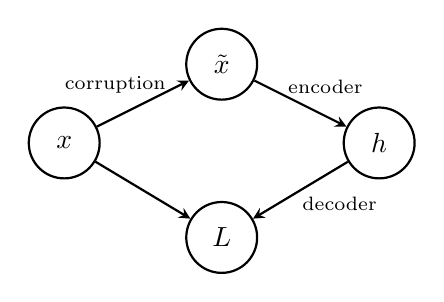
\begin{tikzpicture}[>=stealth,thick]

\node[circle, draw, minimum size=0.9cm] (x) at (0,0) {$x$};
\node[circle, draw, minimum size=0.9cm] (xt) at (2,1) {$\tilde{x}$};
\node[circle, draw, minimum size=0.9cm] (h) at (4,0) {$h$};
\node[circle, draw, minimum size=0.9cm] (L) at (2,-1.2) {$L$};

\draw[->] (x) -- node[midway, above, xshift=-10pt] {\scriptsize corruption} (xt);
\draw[->] (xt) -- node[midway, above, xshift=9pt] {\scriptsize encoder} (h);

\draw[->] (h) -- node[midway, right, xshift=-3pt, yshift=-5pt] {\scriptsize decoder} (L);

\draw[->] (x) -- (L);

\end{tikzpicture}

\caption{Computation graph of a DAE. The clean input $x$ is corrupted into
$\tilde{x}$, encoded into $h$, and decoded to produce a reconstruction that is
compared to $x$ through the loss $\mathcal L$.}
\end{figure}










% ========================
\section{Vincent (2011): Denoising Autoencoders and Score Matching}
% DAE objective, equivalence with score matching, main equations, small-noise limit, key insights.

\subsection{Denoising score matching and its connection to denoising autoencoders}

For simplicity, we denote the score model of our energy-based density by
\[
\psi(x;\theta)\;\approx\;\nabla_x \log p_\theta(x),
\]
so that $\psi(\cdot;\theta)$ is a vector field defined over the data space.  
Denoising Score Matching (DSM) introduces a corrupted observation $\tilde{x}$ obtained from a clean sample $x\sim q(x)$ through a corruption process $q_\sigma(\tilde{x}\mid x)$.  
The corresponding joint distribution factorizes as
\[
q(x,\tilde{x}) = q(x)\, q_\sigma(\tilde{x}\mid x).
\]

\begin{tcolorbox}[colback=gray!5!white,colframe=black,
  title={Denoising Score Matching Objective}]
The Denoising Score Matching (DSM) objective is defined as
\[
J_{\mathrm{DSM}}(\theta)
=
\mathbb E_{q(x,\tilde{x})}
\!\left[
\frac12
\left\|
\psi(\tilde{x};\theta)
-
\nabla_{\tilde{x}} \log q(\tilde{x}\mid x)
\right\|^2
\right],
\]
that is, a mean-squared regression objective where the model predicts the
posterior score $\nabla_{\tilde{x}}\log q(\tilde{x}\mid x)$ from the corrupted
input $\tilde{x}$.
\end{tcolorbox}

This has exactly the structure of a mean squared error regression problem where  
the input is $\tilde{x}$, the prediction is $\psi(\tilde{x};\theta)$, and the regression target is the posterior score $\nabla_{\tilde{x}}\log q(\tilde{x}\mid x)$.\\

Consider now the Gaussian corruption process used in denoising autoencoders:
\[
q(\tilde{x}\mid x)
= \mathcal N(\tilde{x}\mid x,\sigma^2 I).
\]
Since DSM is a least-squares objective in $\psi(\tilde{x};\theta)$, the optimal vector field is the conditional expectation
\[
\psi^\star(\tilde{x})
=
\mathbb E_{q(x\mid \tilde{x})}
\!\left[
\nabla_{\tilde{x}}\log q(\tilde{x}\mid x)
\right].
\]

For Gaussian corruption, the posterior score satisfies
\[
\nabla_{\tilde{x}} \log q(\tilde{x}\mid x)
= \frac{x - \tilde{x}}{\sigma^2}.
\]
Thus,
\[
\psi^\star(\tilde{x})
=
\mathbb E_{q(x\mid\tilde{x})}
\!\left[
\frac{x - \tilde{x}}{\sigma^2}
\right].
\]

This expression makes the denoising interpretation explicit: the optimal vector field $\psi^\star(\tilde{x})$ points, in expectation, from a noisy sample $\tilde{x}$ toward its clean counterpart $x$, scaled by $\sigma^{-2}$.\\

The term $(x-\tilde{x})$ is precisely the reconstruction direction learned by denoising autoencoders, whose objective is to recover $x$ from $\tilde{x}$.\\

A visual illustration is shown in Figure~\ref{fig:scores_fig}, where a one-dimensional data manifold (in red) is corrupted with Gaussian noise.  
The Gaussian corruption kernels around manifold points are shown in green, the noisy samples in grey, and the vector field learned by a denoising autoencoder is represented in blue.  
The resulting field points in the direction of decreasing corruption, back toward the true manifold.\\

\begin{figure}[h!]
\centering
\includegraphics[width=0.7\textwidth]{scores.png}
\caption{One-dimensional data manifold (red), Gaussian corruption kernels (green), noisy samples (grey), and the denoising vector field learned by a DAE (blue).}
\label{fig:scores_fig}
\end{figure}

Vincent~(2011) proved that the DSM objective is equivalent to the ESM and the proof does not depend on the particular form of $q(\tilde{x}\mid x)$ or $q(x)$.

\subsection{An EBM Yielding the DAE Objective}

\begin{tcolorbox}[colback=gray!5!white,colframe=black,title={Connection between DSM and the DAE objective}]
Consider the denoising autoencoder reconstruction loss
\[
L_{\mathrm{DAE}}(\theta)
=
\mathbb E_{q_\sigma(x,\tilde{x})}
\!\left[
\big\|
W^\top \sigma(W\tilde{x}+b) + c - x
\big\|^2
\right],
\]
obtained under Gaussian corruption $q(\tilde{x}\mid x)=\mathcal N(\tilde{x}\mid x,\sigma^2 I)$.\\

For the energy-based model
\[
p(x;\theta)=\frac{1}{Z(\theta)}\exp\!\big(-E(x;\theta)\big),
\qquad
E(x;\theta)
=
-\langle c,x\rangle
-\tfrac12\|x\|^2
+
\sum_{j=1}^{d_h}\!
\operatorname{softplus}(\langle W_j,x\rangle + b_j),
\]
the associated score field satisfies
\[
\psi(x;\theta)
=
\frac{1}{\sigma^2}
\!\left(
W^\top \sigma(Wx+b)+c-x
\right).
\]

Substituting this expression into the denoising score matching loss gives
\[
J_{\mathrm{DSM}}(\theta)
=
\frac{1}{2\sigma^4}\,
L_{\mathrm{DAE}}(\theta).
\]

In other words, minimizing the DSM objective for this EBM is exactly
equivalent to minimizing the denoising autoencoder reconstruction loss.
\end{tcolorbox}


% ========================
\section{Song \& Ermon (2019): Noise-Conditional Score Networks}

\subsection{Motivation: the manifold and low-density problems}

Although Vincent~(2011) showed that denoising autoencoders learn the score of a
smoothed data distribution, using a single fixed noise level~$\sigma$ remains
insufficient for high-dimensional generative modeling.
Real-world data, such as natural images, lie near a low-dimensional manifold in
$\mathbb{R}^d$, where the score~$\nabla_x \log p_{\text{data}}(x)$ is well defined
but becomes unstable in low-density regions.
When sampling with Langevin dynamics, the estimated gradients outside the data
support are unreliable, causing poor mixing or divergence. \\

To address this, Song and Ermon~(2019) proposed to add Gaussian noise to the
data and train the score network across multiple noise levels.
This smoothing makes the data distribution well behaved over all of
$\mathbb{R}^d$, allowing the model to learn stable coarse-scale gradients for
large~$\sigma$ and progressively refine fine details as~$\sigma$ decreases.


\subsection{Noise-conditional network formulation}

The key idea is to make the score model explicitly depend on the noise level~$\sigma$
so that one shared network can learn multiple smoothed versions of the data distribution. \\

Let $\{\sigma_1 > \sigma_2 > \cdots > \sigma_L\}$ denote a geometric sequence of
noise scales.  For each~$\sigma_i$, define the corresponding
Gaussian-smoothed data distribution
\[
q_{\sigma_i}(x)
= \int p_{\text{data}}(x')\,\mathcal N(x \mid x', \sigma_i^2 I)\,dx' .
\]
Each $q_{\sigma_i}$ has full support in~$\mathbb{R}^d$, making its score
well defined everywhere.  Instead of training separate networks for each noise
level, the authors introduced a single model
$s_\theta(x,\sigma)$ that receives both the noisy input~$x$ and the
noise level~$\sigma$ as arguments and is trained to approximate
\[
s_\theta(x,\sigma) \approx \nabla_x \log q_\sigma(x).
\]
Conditioning on~$\sigma$ lets the same network learn score fields at different noise levels:
smoother ones for large~$\sigma$ and more detailed ones for small~$\sigma$.


\begin{tcolorbox}[colback=gray!5!white,colframe=black,
  title={Noise-Conditional Score Network (NCSN)}]
Given a ladder of noise scales $\{\sigma_i\}_{i=1}^{L}$,
a single neural network $s_\theta(x,\sigma)$ is trained to estimate
the score of the Gaussian-smoothed data distribution $q_\sigma$:
\[
s_\theta(x,\sigma) \;\approx\; \nabla_x \log q_\sigma(x).
\]
\end{tcolorbox}

This formulation extends Vincent's denoising autoencoder interpretation.
In Vincent~(2011), training a DAE with Gaussian corruption of variance~$\sigma^2$
makes its reconstruction field~$(r_\theta(x)-x)/\sigma^2$ approximate the score
$\nabla_x \log q_\sigma(x)$ of the data distribution smoothed by Gaussian noise.
Song and Ermon~(2019) generalize this idea by learning a single network
$s_\theta(x,\sigma)$ that predicts these scores jointly for multiple
noise levels~$\sigma$, thereby capturing both coarse and fine structures of the
data manifold.


\subsection{Training objective: denoising score matching (DSM)}

Once the model structure is defined, the next step is to specify how it is trained.
Song and Ermon use a denoising score-matching objective that teaches the network
to recover the exact gradient of the log-density for each noise level. \\

For each fixed noise level~$\sigma$, the network is trained using the
\emph{denoising score-matching} objective
\begin{equation}
\ell(\theta;\sigma)
=\tfrac12\,\mathbb E_{x\sim p_{\text{data}}}
  \mathbb E_{\tilde x\sim\mathcal N(x,\sigma^2 I)}
  \Big[\big\|
    s_\theta(\tilde x,\sigma)
    +\tfrac{\tilde x-x}{\sigma^2}
  \big\|_2^2\Big],
\label{eq:dsm-single}
\end{equation}
where $\tilde x$ denotes a corrupted version of the clean data~$x$.
The vector $(\tilde x-x)/\sigma^2$ corresponds to the exact score of the
Gaussian corruption kernel, so the network learns to reproduce this field from
noisy samples.

Training across all noise scales amounts to minimizing the averaged loss
\begin{equation}
\mathcal L(\theta)
=\frac{1}{L}\sum_{i=1}^{L}
  \lambda(\sigma_i)\,\ell(\theta;\sigma_i),
\qquad
\lambda(\sigma_i)=\sigma_i^2,
\label{eq:dsm-multi}
\end{equation}
where the weighting $\lambda(\sigma)=\sigma^2$ balances gradient magnitudes at
different noise levels and prevents small-$\sigma$ terms from dominating.
This objective is simple, stable, and free of adversarial or likelihood
components; it can be applied to any differentiable network architecture.

\begin{tcolorbox}[colback=gray!5!white,colframe=black,
  title={Key insight}]
By training $s_\theta(x,\sigma)$ to predict the gradient of the
log-density of Gaussian-smoothed data for multiple noise levels,
NCSNs learn a single multi-scale score field that spans from coarse
global structure to fine details.
\end{tcolorbox}

Sampling from these learned scores is performed using the
\emph{annealed Langevin dynamics} procedure described in Section~5.

% ========================
\section{Sampling with Annealed Langevin Dynamics}

\subsection{Motivation}

Once the network has learned score functions $s_\theta(x,\sigma)$ for multiple
noise levels, it can be used to generate new samples.
The goal is to draw samples from the original data distribution
$p_{\text{data}}(x)$ using only its estimated score field.
A natural approach is \emph{Langevin dynamics}, a stochastic process that
iteratively perturbs a particle in the direction of increasing log-density while
adding Gaussian noise to maintain exploration. \\

Standard Langevin dynamics updates a sample~$x_t$ as
\[
x_{t+1} = x_t + \frac{\alpha}{2}\nabla_x \log p(x_t) + \sqrt{\alpha}\,z_t,
\quad z_t \sim \mathcal{N}(0,I),
\]
where $\alpha$ is the step size.
If the score~$\nabla_x \log p(x)$ is exact and $\alpha$ is small enough, this
procedure asymptotically produces samples from~$p(x)$.
However, when applied directly to high-dimensional data, the dynamics tend to
mix very slowly and may get trapped within a single mode.
Song and Ermon~(2019) propose an \emph{annealed} version that leverages the
multi-scale scores learned by the Noise-Conditional Score Network.

\subsection{Annealed Langevin dynamics algorithm}

The central idea is to sample gradually from high noise to low noise.
At large~$\sigma$, the smoothed distribution~$q_\sigma(x)$ is simple and
well connected; as $\sigma$ decreases, the process refines the sample toward
the true data manifold.
For each noise level~$\sigma_i$, the network~$s_\theta(x,\sigma_i)$ provides
an estimate of the score~$\nabla_x \log q_{\sigma_i}(x)$, and Langevin steps
are taken accordingly.

\begin{tcolorbox}[colback=gray!5!white,colframe=black,
  title={Algorithm~1: Annealed Langevin Dynamics \cite{song2019generative}}]
\begin{enumerate}[leftmargin=*,noitemsep]
  \item \textbf{Input:} trained score network $s_\theta(x,\sigma)$,
        noise levels $\sigma_1 > \cdots > \sigma_L$,
        number of iterations $T$ per level, step constant~$\epsilon$.
  \item Initialize $x_0 \sim \mathcal{N}(0, \sigma_1^2 I)$.
  \item \textbf{for} $i = 1, \dots, L$ \textbf{do}
  \begin{enumerate}
    \item Set $\alpha_i = \epsilon \, (\sigma_i / \sigma_L)^2$.
    \item \textbf{for} $t = 1, \dots, T$ \textbf{do}
    \begin{enumerate}
      \item Sample $z_t \sim \mathcal{N}(0,I)$.
      \item Update
      \[
      x \leftarrow x + \frac{\alpha_i}{2} \, s_\theta(x,\sigma_i)
                      + \sqrt{\alpha_i} \, z_t.
      \]
    \end{enumerate}
  \end{enumerate}
  \item \textbf{Output:} final sample $x$.
\end{enumerate}
\end{tcolorbox}

Here the step size~$\alpha_i$ scales proportionally to~$\sigma_i^2$ to maintain
a roughly constant signal-to-noise ratio across levels.
Each stage uses the score field at its own noise level, producing a gradual
denoising trajectory from random Gaussian noise to the data manifold.
The total number of iterations~$L\times T$ is a trade-off between sample
quality and computational cost.

\begin{tcolorbox}[colback=gray!5!white,colframe=black,
  title={Key insight}]
Annealed Langevin dynamics generate samples by successively refining
Gaussian noise using the learned multi-scale score fields.
High-noise levels ensure global coverage, while low-noise levels
restore fine structure consistent with the data distribution.
\end{tcolorbox}

\subsection{Practical considerations}

Empirically, Song and Ermon~(2019) report that many short updates per noise
level yield better results than a few large steps.
Choosing an adequate noise schedule is crucial: $\sigma_1$ must be large
enough to cover the data manifold, and $\sigma_L$ must be small but nonzero to
avoid numerical instability.
They also monitor the norm of $\sigma\,s_\theta(x,\sigma)$ as a diagnostic, which
should remain roughly constant across noise scales if the model is properly
trained.\\

The resulting samples on datasets such as CIFAR-10 and MNIST demonstrate that
score-based generative models can produce realistic images without adversarial
training or explicit likelihood estimation, confirming the effectiveness of
the annealed Langevin framework.


% ========================

\section{A Unifying View: From DAEs to NCSNs}

The transition from Vincent's Denoising Autoencoders to Song and Ermon's Noise-Conditional Score Networks represents a shift from representation learning to full generative modeling.

\subsection{The Bridge}
Vincent (2011) proved that minimizing the reconstruction error of a DAE with noise level $\sigma$ is mathematically equivalent to performing score matching on the smoothed density $q_\sigma(x) = \int p_{\text{data}}(y) \mathcal{N}(x|y, \sigma^2 I) dy$[cite: 156, 164]. Effectively, the "denoising vector" learned by the autoencoder points towards the mode of the data distribution[cite: 129].

However, a single DAE trained with a fixed, small $\sigma$ fails as a generative model. As noted by Song and Ermon (2019), real-world data resides on low-dimensional manifolds[cite: 363]. Ideally, we want $\sigma \to 0$, but in this limit, the score is undefined in the ambient space, and the training signal vanishes in low-density regions[cite: 300, 301]. Conversely, a large $\sigma$ makes score estimation stable but destroys fine data details.

\subsection{The Multi-Scale Solution}
The key innovation of the NCSN framework is to accept this trade-off and utilize \textit{all} noise levels. Instead of training separate DAEs, Song and Ermon train a single network $s_\theta(x, \sigma)$ conditioned on the noise level[cite: 459].
\begin{itemize}
    \item \textbf{At high $\sigma$:} The noise "fills" the low-density regions, allowing the network to learn global structure and mix between distant modes[cite: 447].
    \item \textbf{At low $\sigma$:} The network refines the samples, recovering the sharp details of the data manifold[cite: 508].
\end{itemize}
This transforms the DAE from a feature extractor into a multi-scale gradient estimator capable of guiding a sampling process from pure noise to realistic data.


% ========================
\section{Experimental Results and Observations}

We evaluate the efficacy of Noise-Conditional Score Networks (NCSN) combined with Annealed Langevin Dynamics. The experiments focus on two main aspects: the ability to generate high-fidelity samples on complex image datasets and the ability to mix between separated modes in a distribution.

\subsection{Image Generation Performance}
[cite_start]The model was trained on MNIST, CelebA, and CIFAR-10 datasets[cite: 40]. [cite_start]The generated samples demonstrate that score-based models can produce high-quality images comparable to modern likelihood-based models and GANs without requiring adversarial training[cite: 11, 41].

Quantitative evaluation on CIFAR-10 highlights the effectiveness of the method:
\begin{itemize}
    [cite_start]\item \textbf{Inception Score:} The NCSN achieves a score of \textbf{8.87}, setting a new state-of-the-art for unconditional generative models at the time of publication[cite: 11, 42].
    [cite_start]\item \textbf{FID Score:} The model achieves a Fréchet Inception Distance of \textbf{25.32}, which is competitive with leading GAN architectures like SNGAN[cite: 42, 276].
\end{itemize}

\subsection{Mode Mixing (The Toy Experiment)}
A crucial observation from \cite{song2019} is the failure of standard Langevin dynamics to mix properly when modes are separated by low-density regions.
\begin{itemize}
    [cite_start]\item \textbf{Standard Langevin:} When applied to a mixture of two Gaussians with disjoint supports, standard sampling fails to recover the correct relative weights of the modes, often becoming trapped in a single mode[cite: 124, 133].
    \item \textbf{Annealed Langevin:} By starting with large noise ($\sigma_1$), the sampler bridges the low-density gap. [cite_start]As the noise level is annealed down to $\sigma_L$, the method faithfully recovers the relative weights of the mixture distribution[cite: 171, 243].
\end{itemize}

\subsection{Representation Learning}
Beyond generation, the score network learns semantic representations of the data. [cite_start]This is evidenced by image inpainting experiments, where the model successfully reconstructs occluded parts of an image using the learned gradient fields, demonstrating it has captured the underlying structure of the data rather than simply memorizing training examples[cite: 12, 278].
% ========================
\section{Practical Notes & Limitations}

\subsection{Hyperparameters and Stability}
Implementing NCSNs requires careful tuning of the noise "ladder" $\{\sigma_i\}_{i=1}^L$:
\begin{itemize}
    \item \textbf{Geometric Sequence:} The noise levels are chosen as a geometric progression where $\frac{\sigma_1}{\sigma_2} = \dots = \frac{\sigma_{L-1}}{\sigma_L} > 1$[cite: 457]. $\sigma_1$ must be large enough to cover the data variance, while $\sigma_L$ should be small enough to be invisible to the human eye[cite: 458].
    \item \textbf{Step Size ($\alpha$):} For the annealed Langevin dynamics, the step size $\alpha_i$ must scale with the noise variance. Song and Ermon propose $\alpha_i \propto \sigma_i^2$ to maintain a constant signal-to-noise ratio throughout the sampling process[cite: 509].
\end{itemize}

\subsection{Limitations}
While avoiding adversarial training is a major advantage, the framework has limitations:
\begin{itemize}
    \item \textbf{Computational Cost:} The sampling process is iterative (e.g., $T=100$ steps per noise level [cite: 522]), which is significantly slower than single-pass generators like GANs.
    \item \textbf{Bias:} As noted by Vincent (2011), the score estimator is biased when $\sigma > 0$. While beneficial for stability, it means we are theoretically sampling from a slightly smoothed distribution rather than the exact $p_{\text{data}}$[cite: 187].
\end{itemize}

% ========================
\section{Conclusion}

We have presented a coherent narrative linking Denoising Autoencoders to modern score-based generative models. Vincent (2011) laid the theoretical groundwork by identifying the connection between denoising objectives and score matching[cite: 164]. Song and Ermon (2019) resolved the geometric instabilities of the single-noise approach by introducing noise-conditional networks and annealed sampling[cite: 281]. This lineage demonstrates that learning to "undo" noise at multiple scales is equivalent to learning the gradient of the data distribution, providing a stable and principled foundation for generative modeling without adversarial objectives.
% ========================
\bibliographystyle{plain} % or 'alpha', 'unsrt', etc.
\bibliography{references} % This tells LaTeX to look for references.bib
% ========================
\appendix
\section{Derivation Snippets}
% Optional small derivations from Vincent (2011).

\section{Glossary of Notation}
% List of key symbols and definitions.

\end{document}
